\documentclass[12pt,a4paper]{article}
\usepackage[utf8]{inputenc}
\usepackage[T1]{fontenc}
\usepackage{fontspec}
\setmainfont{Times New Roman}
\newfontfamily\hackfont{Hack}
\usepackage{titlesec}
\usepackage{fancyhdr}
\usepackage{listings}
\usepackage{xcolor}
\usepackage{graphicx}
\usepackage{longtable}
\usepackage{caption}
\usepackage{hyperref}
\usepackage{setspace}
\usepackage{geometry}
\geometry{a4paper, margin=1in}
\hypersetup{colorlinks=true, linkcolor=blue, urlcolor=blue}
\renewcommand{\contentsname}{Table of Contents}

\pagestyle{fancy}
\fancyhf{} 							% Header Middle
\rhead{VLSI Design Lab}
\lhead{Lab-05: Stick Diagram}
\rfoot{\thepage}

\begin{document}

\begin{titlepage}					% Cover Start
\begin{center}
    
\includegraphics[width=0.35\textwidth]{logo.png} \\
    \vspace{0.5cm}
    \textbf{\Huge \textcolor{cyan}{NOTRE DAME} \textcolor{cyan}{UNIVERSITY}} \\
    \vspace{0.5cm}
    \textbf{\Huge \textcolor{orange}{BANGLADESH}} \\
    
    \vspace{0.9cm}
    \textbf{\Huge \underline{VLSI Design Lab Report-05}} \\
    
    \vspace{1.5em}
    \begin{flushleft}
    	\textbf{\Large Course Code: CSE-4218} \\
		\vspace{0.3cm}        
        \textbf{\Large Course Title: VLSI Design Lab} \\
        \vspace{0.3cm}
        \textbf{\Large Experiment Name: Stick Diagram in MICROWIND2} \\        
    \end{flushleft}
    
    \vspace{1em}
    \begin{flushleft}
        \textbf{\Huge \textcolor{blue}{Submitted by:}} \\
        \vspace{0.3cm}
        \textbf{\Large Name: Istiak Alam} \\
        \vspace{0.3cm}
        \textbf{\Large ID: 0692230005101005} \\
		\vspace{0.3cm}        
        \textbf{\Large Batch: CSE-20} \\
        \vspace{0.5cm}
        \textbf{\Large Submission Date: }{\Large \textbf{\today}\par}
    \end{flushleft}
    \vfill
    \begin{flushleft}
        \textbf{\Huge \textcolor{blue}{Submitted to:}} \\
        \vspace{0.3cm}
        \textbf{\Large Nafisa Tabassum,} \\
        \vspace{0.3cm}
        \textbf{\Large Lecturer, Dept. of CSE} \\
        \vspace{0.3cm}
        \textbf{\Large Notre Dame University Bangladesh}
    \end{flushleft}
\end{center}
\end{titlepage}						% Cover End

\tableofcontents
\thispagestyle{empty}
\clearpage
\pagenumbering{arabic}

\section*{\center Abstract}
This laboratory experiment focuses on the implementation of CMOS stick diagrams using the Microwind2 layout design tool. Stick diagrams for fundamental logic gates, including the 2-input NAND gate, 2-input NOR gate, and 1-input inverter, were developed following standard VLSI layout conventions. The diagrams represent simplified layout structures using color-coded layers such as polysilicon, diffusion, and metal interconnections. The primary objective of this experiment is to understand the physical representation of CMOS circuits and the relationship between schematic design and layout realization. The resulting stick diagrams provide a compact and technology-independent view of circuit structures, which is essential for efficient VLSI design.



\section{Introduction}
In VLSI design, the transition from schematic-level representation to physical layout is a critical step in the design process. Stick diagrams serve as an intermediate abstraction that simplifies the visualization of circuit layouts without considering exact dimensions. These diagrams use standardized color codes to represent different layers such as polysilicon, diffusion regions, and metal interconnections.

Microwind2 is a layout design tool that allows designers to implement and simulate CMOS circuits at the physical level. In this experiment, stick diagrams of basic logic gates were implemented to understand layout organization, transistor placement, and interconnection strategies. The study of stick diagrams helps in developing an understanding of design rules, layout optimization, and area-efficient circuit implementation in VLSI systems.


\section{Objective}
The objectives of this laboratory experiment are as follows:
\begin{itemize}
    \item To understand the concept and importance of stick diagrams in VLSI layout design.
    \item To implement stick diagrams of basic CMOS logic gates using Microwind2.
    \item To represent transistor-level circuits using simplified, technology-independent layouts.
    \item To analyze the arrangement of polysilicon, diffusion, and metal layers in CMOS design.
    \item To develop a clear understanding of the relationship between schematic design and physical layout.
\end{itemize}


\newpage
\section{1 Input Inverter (NOT Gate)}
The inverter, also known as a NOT gate, is the most fundamental logic gate in digital design. It produces the logical complement of the input signal. In CMOS technology, the inverter is implemented using one PMOS transistor in the pull-up network and one NMOS transistor in the pull-down network. The stick diagram represents this structure using polysilicon for gate control, diffusion regions for source and drain, and metal layers for interconnections. The inverter serves as the basic building block for more complex CMOS circuits.

\subsection*{Stick Diagram}
\begin{figure}[!h]
\centering
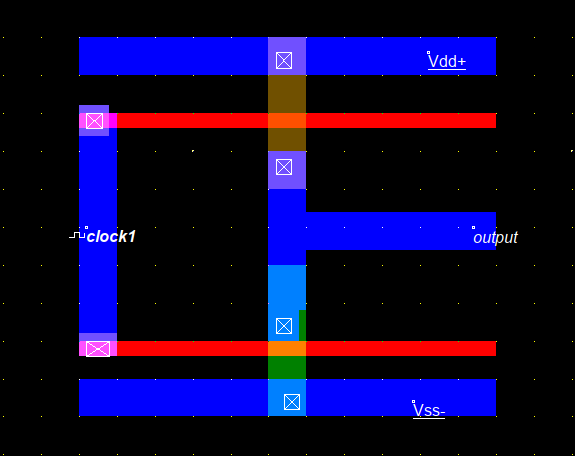
\includegraphics[width=1\textwidth]{Inverter.png}
\caption{Stick Diagram of Inverter (NOT Gate) in MICROWIND2}
\end{figure}
\newpage
\subsection*{Output}
\begin{figure}[!h]
\centering
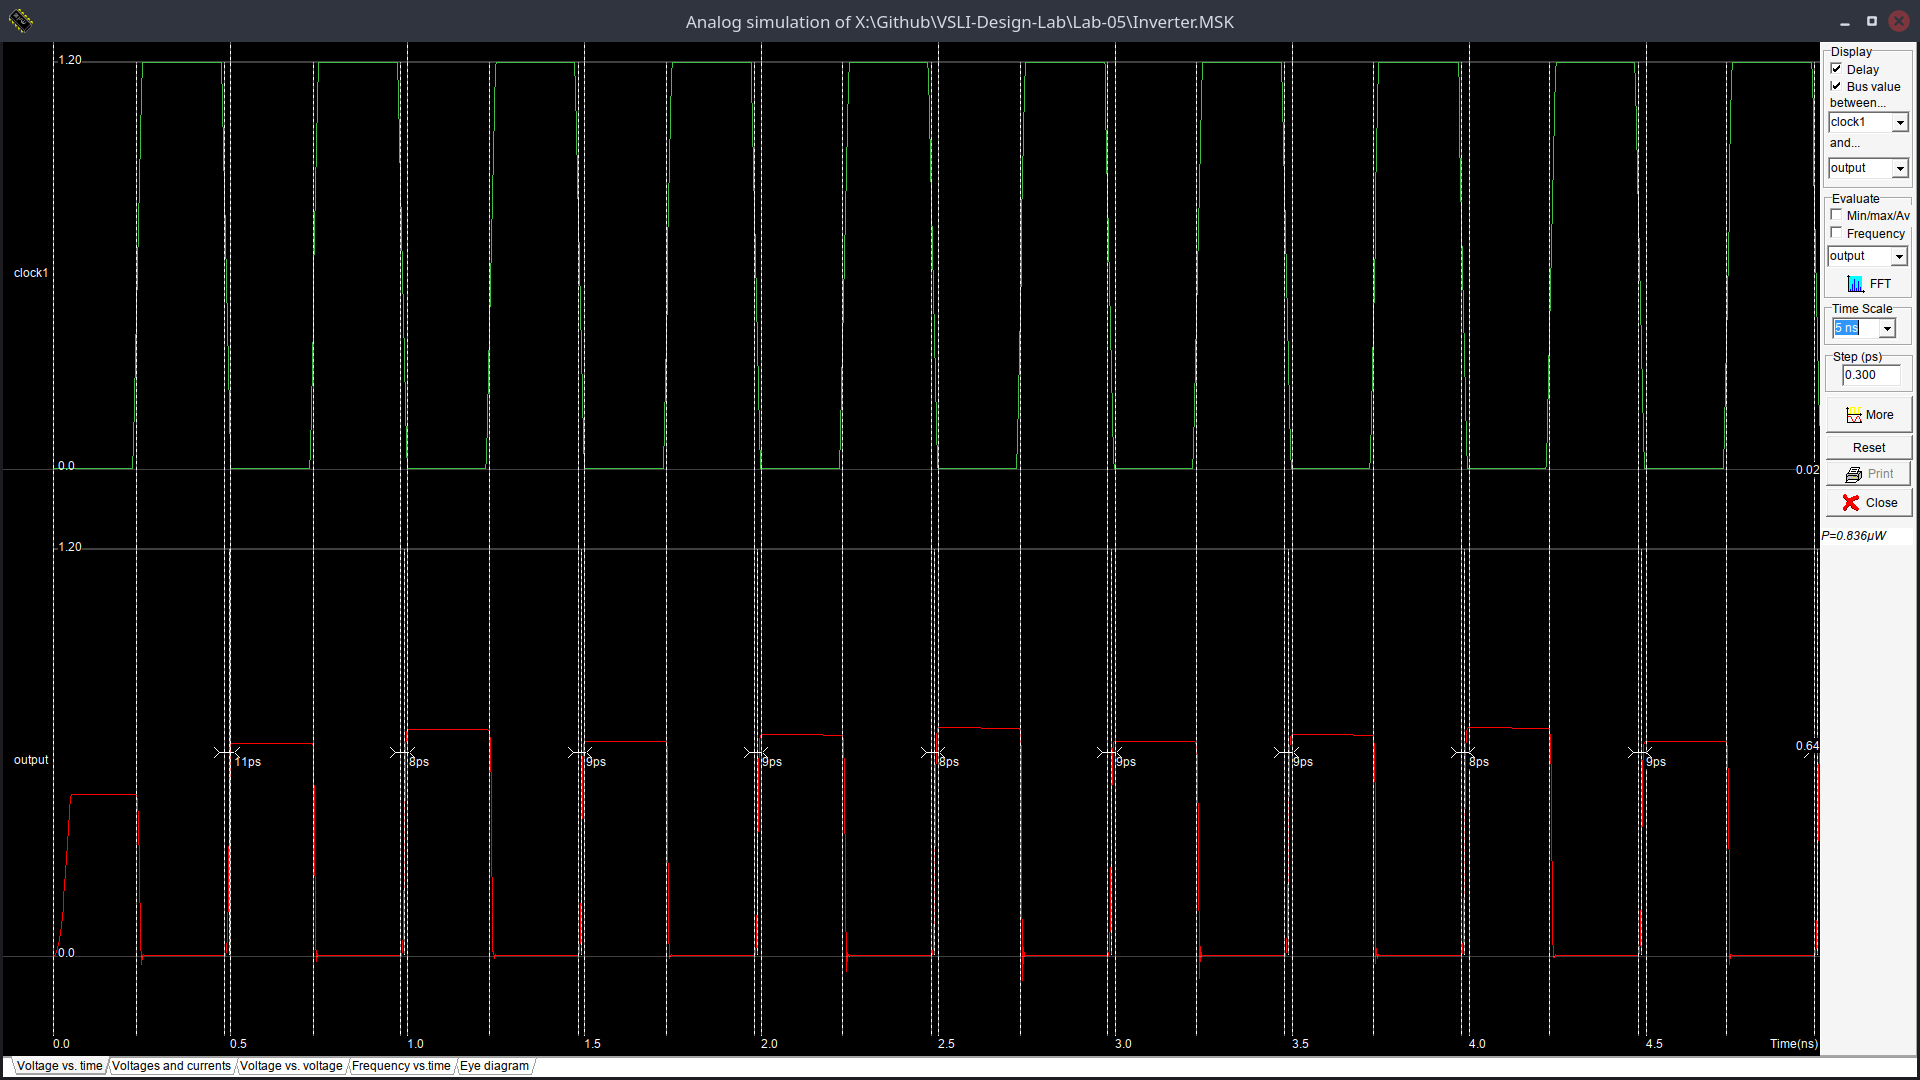
\includegraphics[width=1\textwidth]{Inverter-Out.png}
\caption{Analog Simulation of Inverter (NOT Gate)}
\end{figure}

From the output waveform, it is observed that the inverter produces the exact complement of the input signal. When the input is at logic HIGH, the NMOS transistor conducts and pulls the output to logic LOW. Conversely, when the input is at logic LOW, the PMOS transistor conducts and pulls the output to logic HIGH. The transition between output states occurs immediately following the input change, demonstrating correct switching behavior. The observed output confirms the proper operation of the CMOS inverter as expected from its theoretical truth table.





\newpage
\section{2 Input NAND Gate}
A 2-input NAND gate is a fundamental universal logic gate that produces a logic LOW output only when both inputs are logic HIGH. In CMOS layout design, the NAND gate is implemented using two NMOS transistors connected in series in the pull-down network and two PMOS transistors connected in parallel in the pull-up network. The stick diagram represents this structure using simplified layer representations such as polysilicon for gates, diffusion for active regions, and metal for interconnections.

\subsection*{Stick Diagram}
\begin{figure}[!h]
\centering

\includegraphics[width=1\textwidth]{2in-NAND.png}
\caption{Stick Diagram of 2in-NAND Gate in MICROWIND2}
\end{figure}
\newpage
\subsection*{Output}
\begin{figure}[!h]
\centering
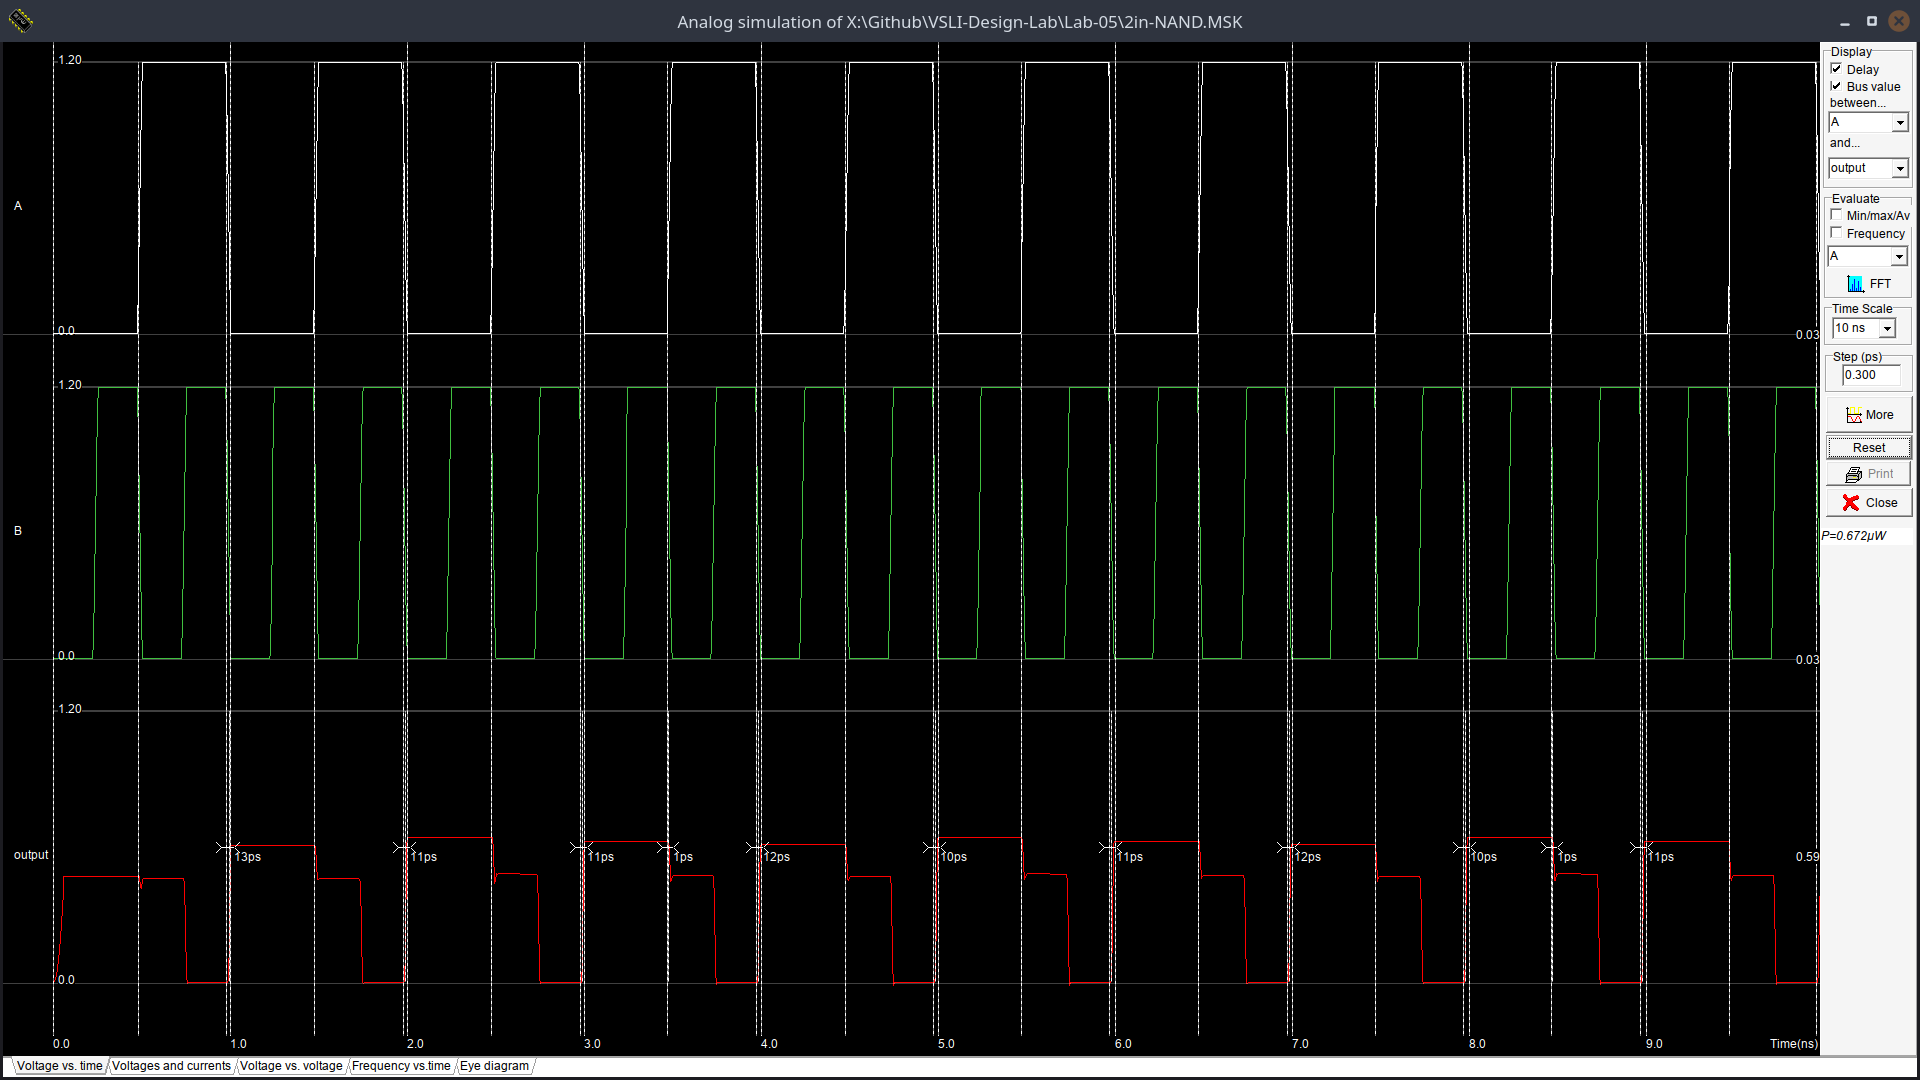
\includegraphics[width=1\textwidth]{2in-NAND-Out.png}
\caption{Analog Simulation of 2in-NAND Gate}
\end{figure}

\subsection*{Observation}
From the simulation results obtained in Microwind2, it is observed that the output remains at logic HIGH for all input combinations except when both inputs are HIGH. When inputs A and B are simultaneously at logic HIGH, the series NMOS transistors in the pull-down network conduct, creating a path to ground and forcing the output to logic LOW. For all other input conditions, at least one PMOS transistor in the pull-up network remains active, maintaining the output at logic HIGH. The observed output waveform matches the expected truth table of a 2-input NAND gate, confirming the correctness of the stick diagram implementation.





\newpage
\section{2 Input NOR Gate}
The 2-input NOR gate is a fundamental digital logic gate that produces a logic HIGH output only when both inputs are at logic LOW. In CMOS implementation, the NOR gate is realized using parallel NMOS transistors in the pull-down network and series PMOS transistors in the pull-up network. In the stick diagram representation using Microwind2, different layers such as polysilicon, diffusion, and metal are arranged according to standard layout conventions to form the required transistor connections. The stick diagram provides a simplified visualization of the physical layout without considering exact dimensions.
\subsection*{Stick Diagram}
\begin{figure}[!h]
\centering

\includegraphics[width=1\textwidth]{2in-NOR.png}
\caption{Stick Diagram of 2in-NOR Gate in MICROWIND2}
\end{figure}
\newpage
\subsection*{Output}
\begin{figure}[!h]
\centering
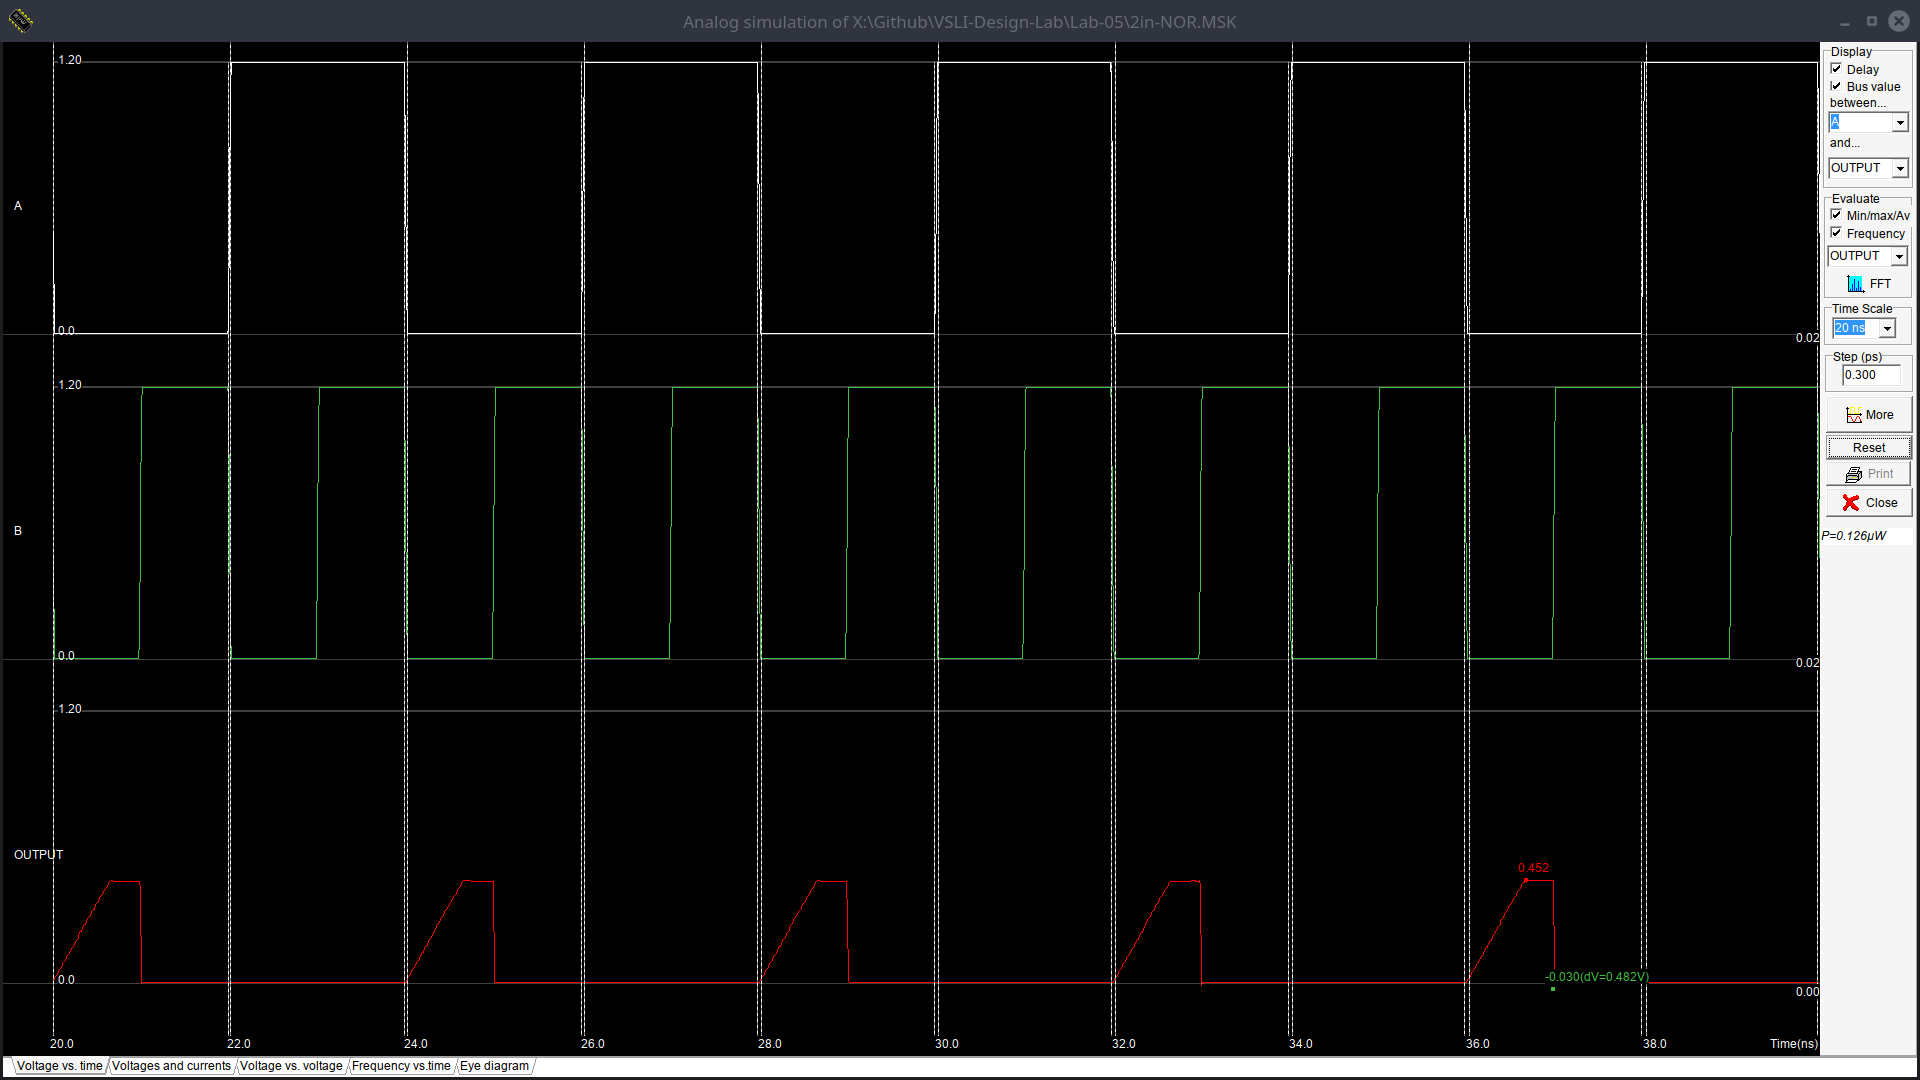
\includegraphics[width=1\textwidth]{2in-NOR-Out.png}
\caption{Analog Simulation of 2in-NOR Gate}
\end{figure}

\subsection*{Observation}
From the simulation results, it is observed that the output of the 2-input NOR gate remains logic HIGH only when both inputs are LOW (0,0). For all other input combinations, i.e., when any one or both inputs are HIGH, the output becomes logic LOW. The output waveform clearly reflects this behavior, showing a HIGH level only in the absence of input signals. This verifies the correct implementation of the NOR logic function in the stick diagram using Microwind2.

% =====================================================
\section{Conclusion}
The simulation outputs verified that each gate produces the expected logical behavior according to its truth table. The stick diagrams provided a simplified yet effective representation of the physical layout, helping to visualize transistor placement and interconnections without considering exact geometrical dimensions. It was also observed that proper alignment of layers is essential to ensure correct circuit functionality.\\
In this laboratory experiment, stick diagrams of basic CMOS logic gates were successfully designed and implemented using Microwind2. The study demonstrated how schematic-level logic can be translated into physical layout representations using simplified diagrammatic techniques.




\end{document}